%Micah Chambers

\documentclass{beamer}
\usepackage[orientation=landscape,size=custom,width=16,height=10,scale=0.5,debug]{beamerposter} 

\mode<presentation>
{
  \usetheme{VT}
  % or ...

  \setbeamercovered{transparent}
  % or whatever (possibly just delete it)
}

\usefonttheme[onlylarge]{structurebold}
\usecolortheme{crane}
\setbeamerfont*{frametitle}{size=\normalsize,series=\bfseries}
\setbeamertemplate{navigation symbols}{}
\setbeamercovered{transparent}


\usepackage[english]{babel}
% or whatever

\usepackage[latin1]{inputenc}
% or whatever

\usepackage{graphics}
%\usepackage{times}
\usepackage[T1]{fontenc}
\usepackage[small]{caption}
\usepackage{algorithmic}

\title{BOLD Parameter Estimation using Sequential Monte Carlo Methods}

%\subtitle{}

\author{Micah Chambers}

\institute {Virginia Tech Bioimaging Systems Lab}

\subject{Medical Imaging}

% If you have a file called "university-logo-filename.xxx", where xxx
% is a graphic format that can be processed by latex or pdflatex,
% resp., then you can add a logo as follows:

\pgfdeclareimage[width=1.5cm]{university-logo}{logo}
\logo{\pgfuseimage{university-logo}}


% If you wish to uncover everything in a step-wise fashion, uncomment
% the following command: 

%\beamerdefaultoverlayspecification{<+->}


\begin{document}
\begin{frame}
  \titlepage
\end{frame}

\begin{frame}{Outline}
  \tableofcontents
  % You might wish to add the option [pausesections]
\end{frame}

\section{FMRI Review}
\begin{frame}{The BOLD Response}
\begin{figure}
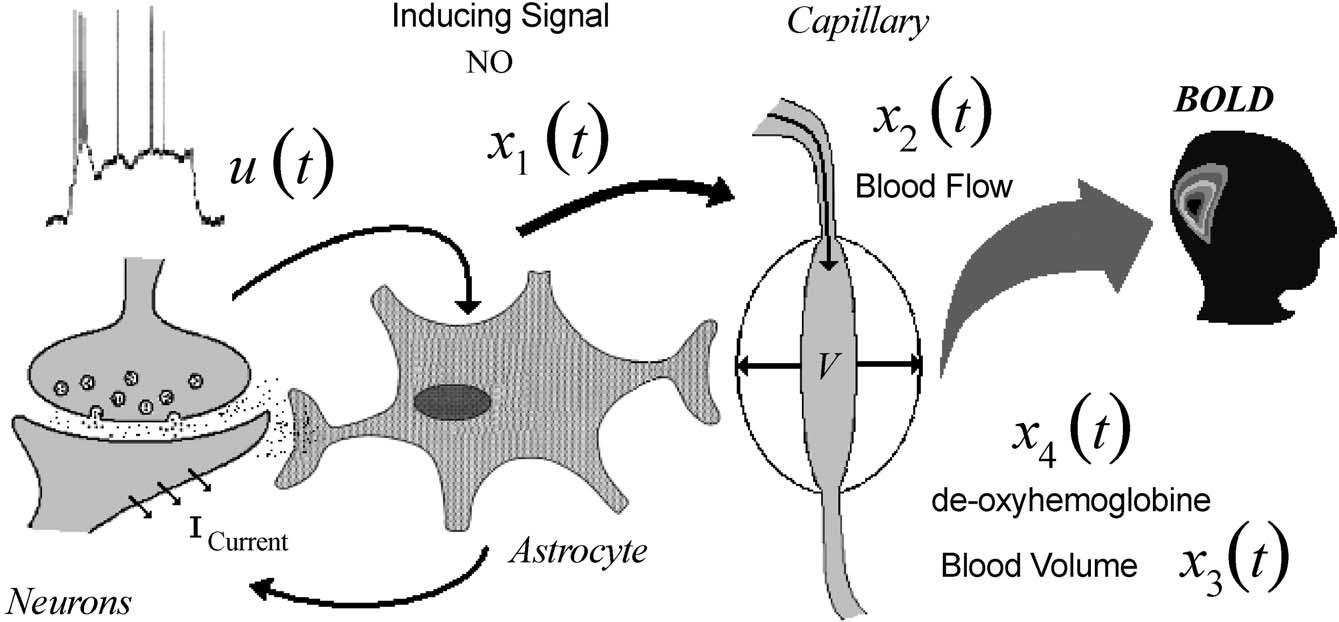
\includegraphics[scale=.23]{model}
\caption{
    \tiny
    \cite{nonlinearfiltering}
}
\end{figure}
\end{frame}

\begin{frame}{BOLD Signal Properties}
  \begin{itemize}
    \item Exact variables and parameters are unknown and are
        difficult to calculate.
    \item Significant Amount of Lag between activation
        and a measurable output - can be as much as 8 seconds.
    \item Slow Temporal Resolution
    \item Noise characterized by brownian motion, which clashes with low 
        frequency elements.
    \begin{center}
    \includegraphics[width=10cm,height=4cm]{signal_fft.pdf}
    \end{center}
  \end{itemize}
\end{frame}

\begin{frame}{Preprocessing}
  \begin{itemize}
    \item Low Pass Filter (Gaussian Filter, not recommended)
    \item Drift Removal (not always performed)
    \begin{itemize}
        \item High Pass Filter
        \item Linear 
        \item Quadratic
        \item Wavelet 
        \item Spline (Which I am using)
    \end{itemize}
  \end{itemize}
  \begin{figure}
    \includegraphics[width=10cm]{detrending_effect.png}
    \caption{
        \tiny
        \cite{detrending}
    }
  \end{figure}
\end{frame}

\section{Statistical Parametric Mapping}
\begin{frame}{Method}
  \begin{figure}
    \includegraphics[width=11cm]{glm_pipeline.png}
    \caption{
        \tiny
        \cite{spm_pipeline}
    }
  \end{figure}
\end{frame}

\begin{frame}{Limitations}
\begin{columns}
  \column{2.5in}
  \begin{itemize}
    \item Linear, for a signal which is known to be nonlinear
    \item Essentially the weighted sum of a set of "expected" responses.
    \item Parametric
    \begin{itemize}
        \item Forced to make assumptions about underlying distributions
        \item No time-scaling.
    \end{itemize}
  \end{itemize}
  \column{3in}
  \begin{figure}
    \includegraphics[width=2.5in]{glm.png}
    \caption{
        \tiny
        \cite{spm_pipeline}
    }
  \end{figure}
\end{columns}
\end{frame}

\section{Nonlinear Regression}
\begin{frame}{Equations}
  \begin{itemize}
    \item Normalized Cerebral Blood Flow:
    $$\ddot{f}(t) = \epsilon u(t) - \dot{f}(t)/\tau_s - (f(t)/\tau_f - 1)$$
    \item Normalized Cerebral Blood Volume:
    $$\dot{v}(t) = (1/\tau_0)( f(t) - v(t) ^ {1/\alpha}) $$
    \item Normalized Deoxyhaemoglobin Content:
    $$\dot{q}(t) = \frac{1}{\tau_0}\left(\frac{f(t)(1- (1-E_0)^{1/f(t)})}{E_0} - 
            \frac{q(t)}{v(t)^{1-1/\alpha}}\right)$$
    \item Hemodynamic Response - BOLD Signal
    $$y(t) = V_0(a_1( 1 - Q(t)) - a_2(1 - V(t)))$$
  \end{itemize}
\end{frame}

\begin{frame}{Model Comparison}
  \begin{figure}
    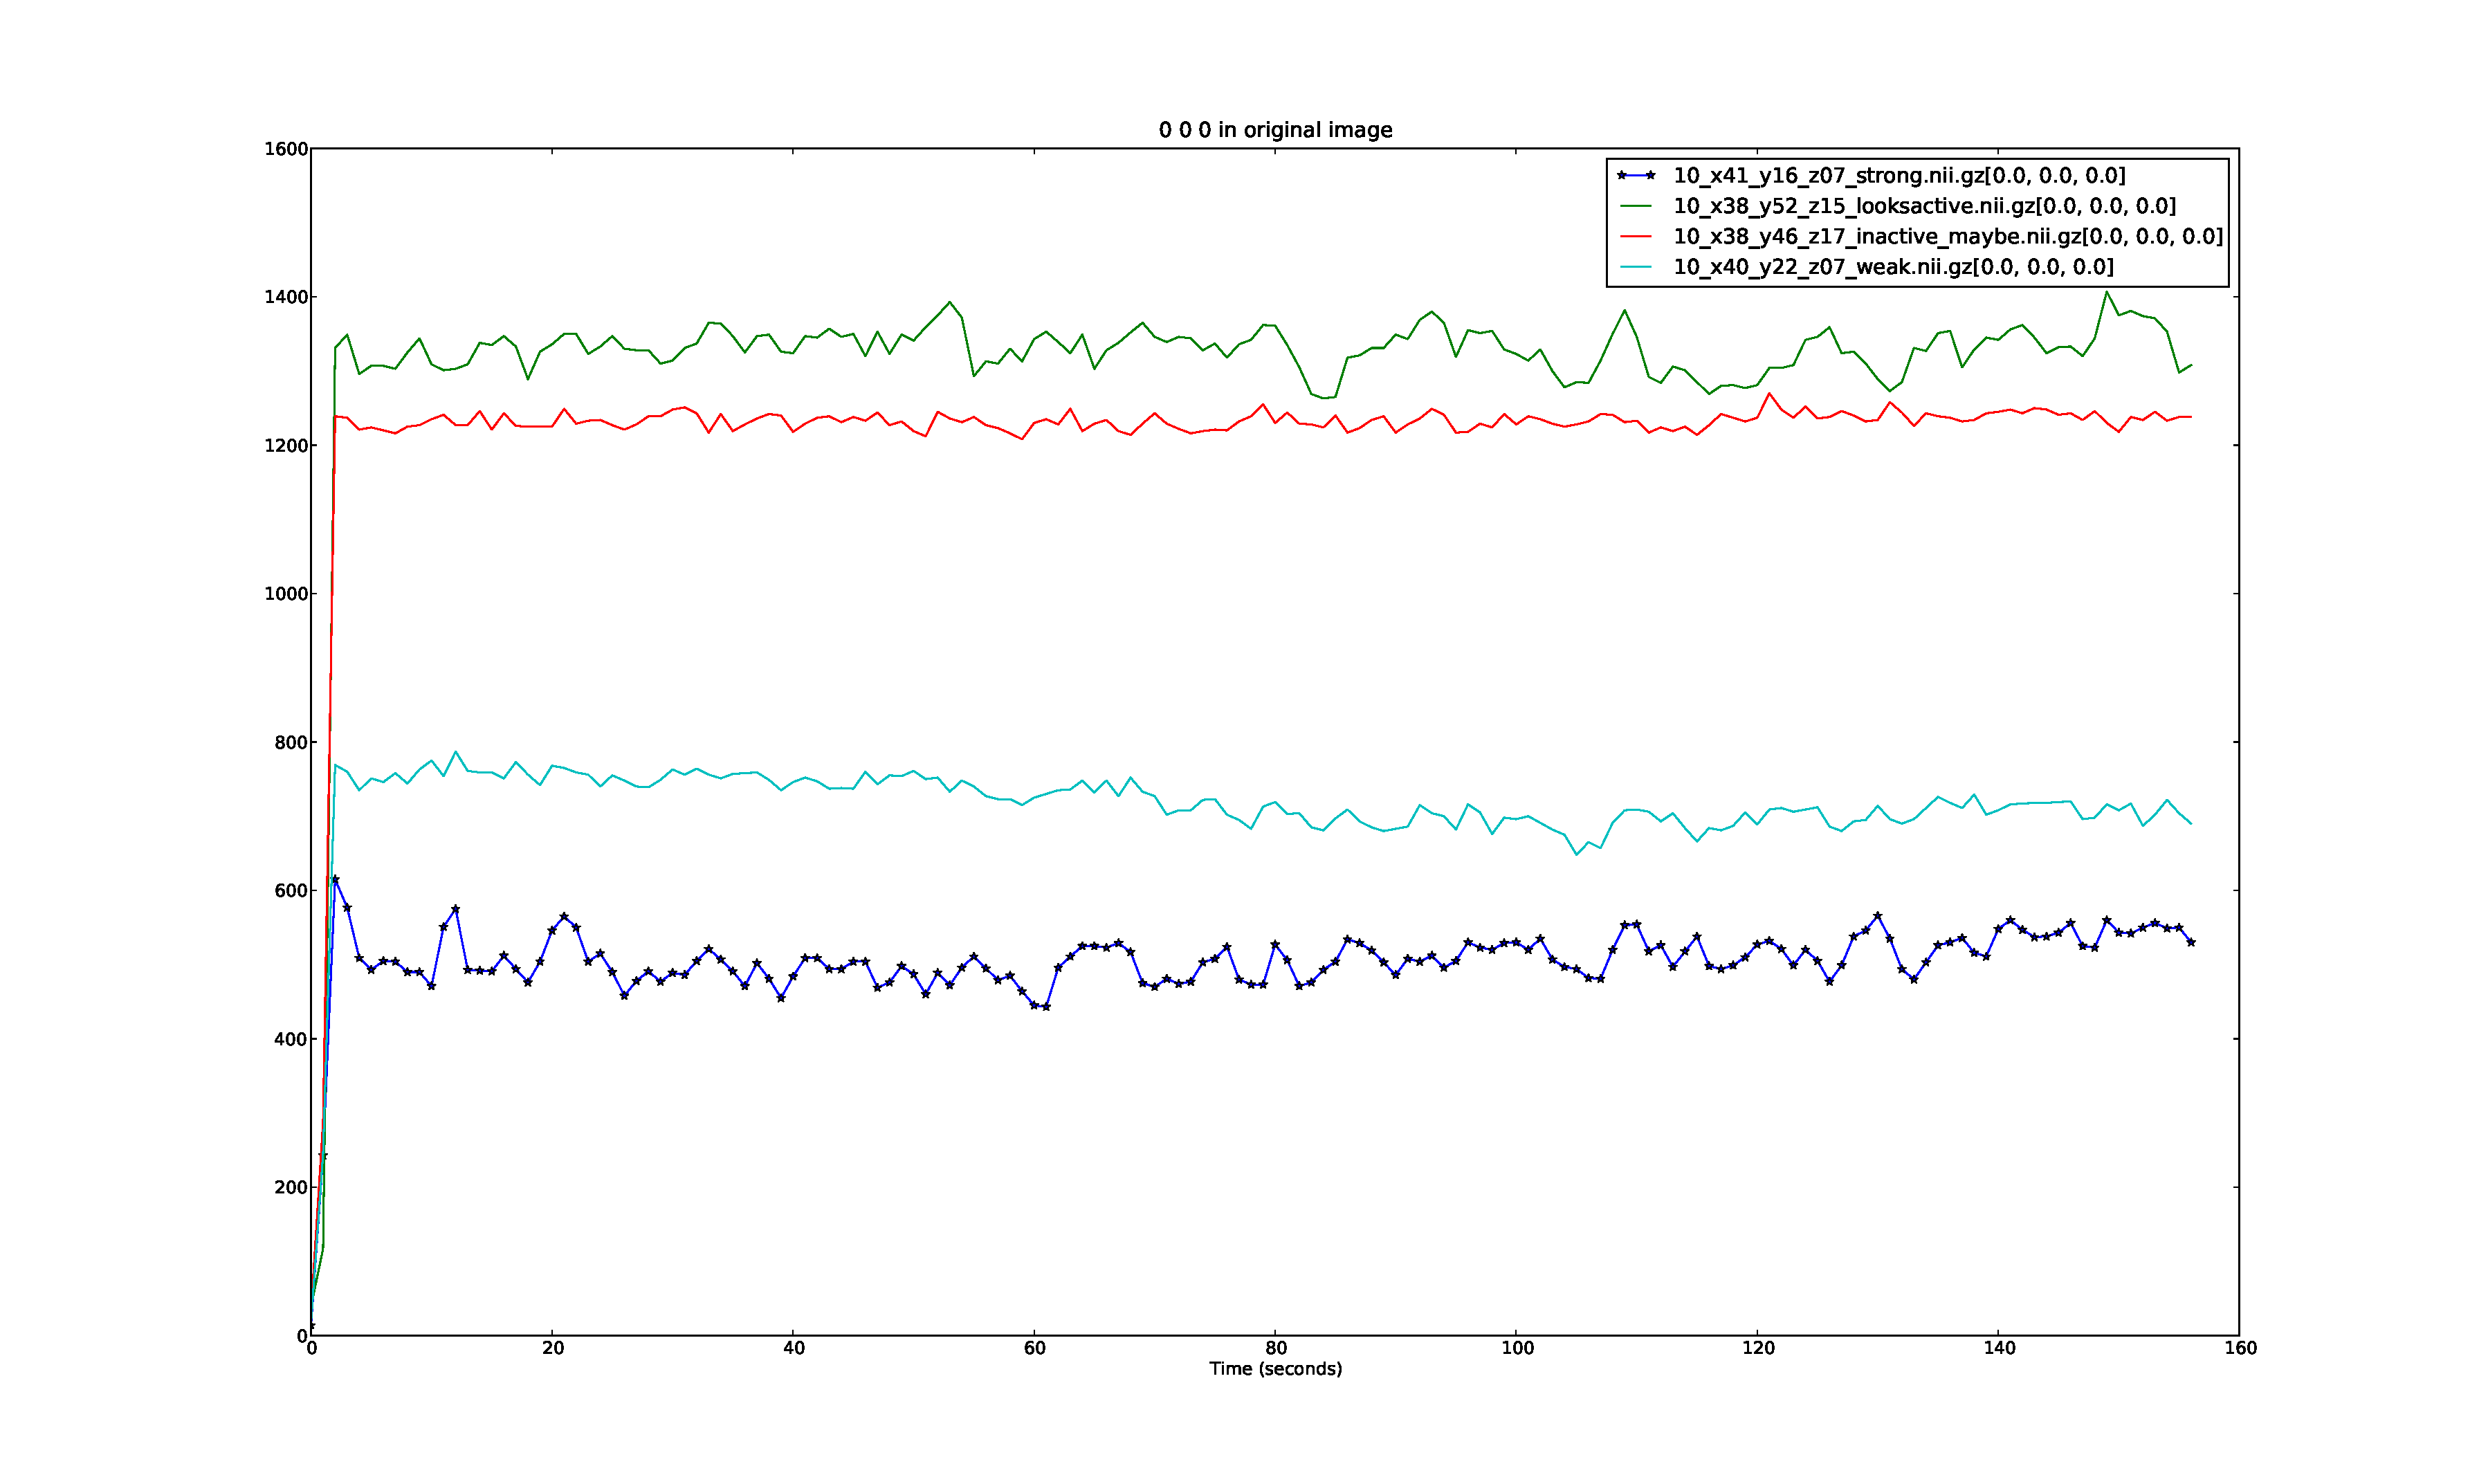
\includegraphics[width=5in,height=2.4in]{comparison.png}
    \caption{
        \tiny
        \cite{comparison}
    }
  \end{figure}
\end{frame}

\section{Parameter Identification}
\begin{frame}{Particle Filters}
\begin{itemize}
    \item Non-parametric, no assumptions are violated
    \item Model based, fit parameters to input, constrained by physical variables
    \item Fits a mixture PDF to the posterior of all parameters
    \item Non-trivial computation cost
    \item I use a Regularized Particle Filter
    \begin{enumerate}
        \item Regularized Re-sampling prevents particles from de-generating into a 
            small number of unique particles
        \item Allows distributions to move more freely
    \end{enumerate}
\end{itemize}
\end{frame}

\begin{frame}{Particle Filter}
    \begin{columns}
    \column{1.8in}
    \begin{itemize}
        \item $S_t = \{p_{0,t}, ... , p_{N,t}\}$, the set of particles
        \item $w_{i,t}$, weight of particle $p_{i,t}$
        \item $y_t$, measurement at time $t$, there is not a $y_t$ for every $t$.
        \item $f(p_{i,t},y_t)$, weighting function 
        \item $s(p_{i,t})$, step function 
    \end{itemize}
    \column{3.2in}
    \begin{algorithmic}
     \STATE Draw $S_0$ from prior distribution 
     \FOR{$t = 0:t_{step}:t_{end}$}
        \FOR{each $p_{i,t-1} \in S_{t-1}$}
           \STATE $p_{i,t} = s(p_{i,t-1})$ 
           \IF{There is a measurement at time $t$}
               \FOR{every $p_{i,t}$}
                    \STATE $w_{i,t} = w_{i,t-1}f(p_{i,t},y_t)$
               \ENDFOR 
               \STATE Resample if weights are unevenly distributed\\
           \ENDIF
        \ENDFOR
     \ENDFOR
%                    \item If a weights are not evenly distributed enough, then resample
     \end{algorithmic}
     \end{columns}
\end{frame}

\subsection{Single-Region}
\begin{frame}{Single Timeseries Results}
  \begin{figure}
    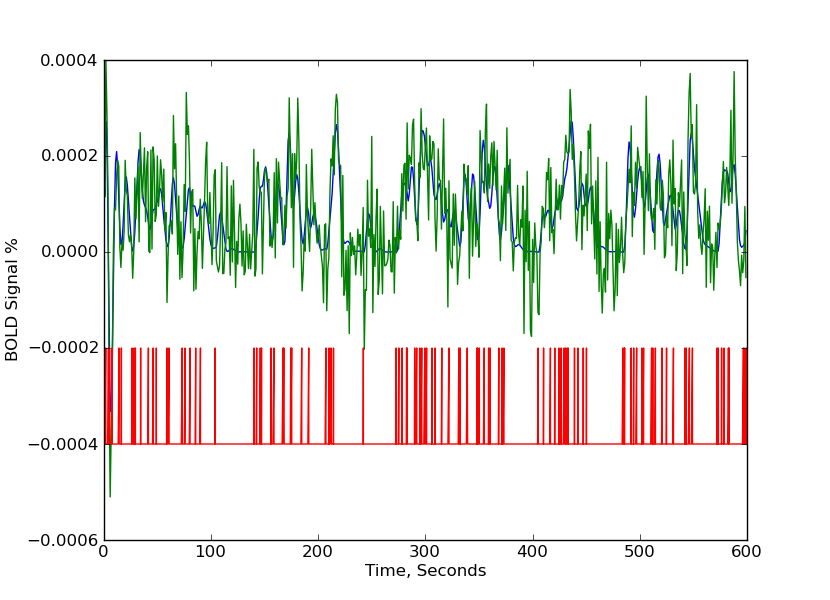
\includegraphics[height=3in]{noise.png}
  \end{figure}
\end{frame}

\begin{frame}{Single Timeseries Results, Measurement Convergence}
  \begin{figure}
    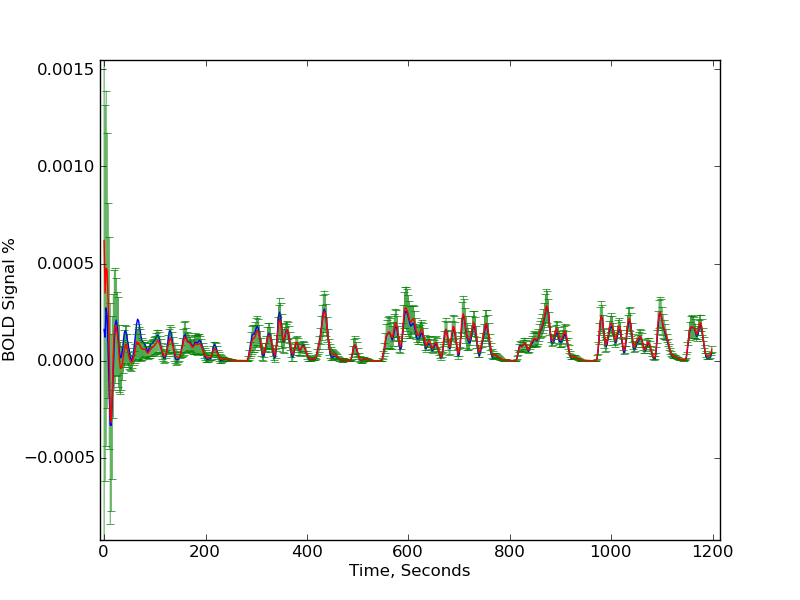
\includegraphics[height=3in]{bold.png}
  \end{figure}
\end{frame}

\begin{frame}{Single Timeseries Results, State Convergence}
  \begin{figure}
    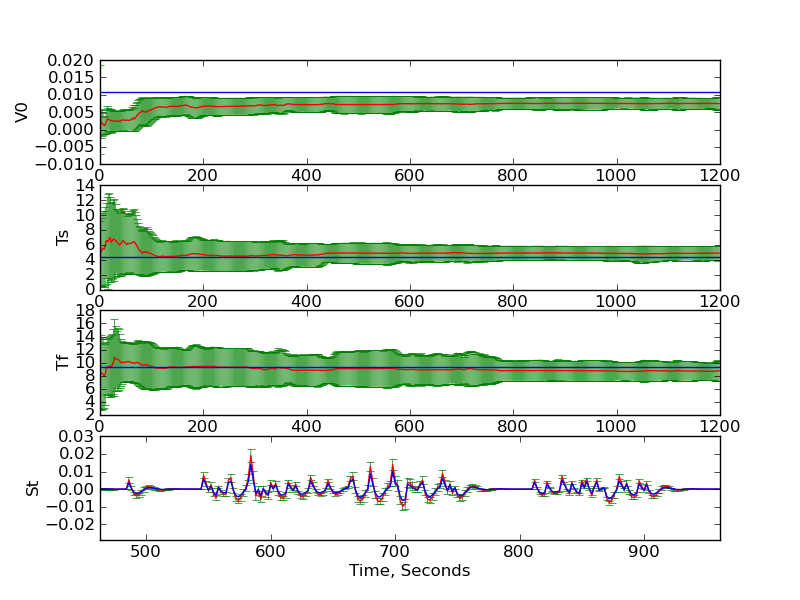
\includegraphics[height=3in]{state.png}
  \end{figure}
\end{frame}

\begin{frame}{Factors Affecting Convergence}
    \begin{enumerate}
        \item Weighting function
            \begin{itemize}
                \item Needs to be continuous and defined for any input, should go to 0
                \item Too wide a weighting function results in under-sensitivity, 
                            slow or no convergence
                \item Too thin a weighting function reduces robustness to noise
            \end{itemize}
        \item How often re-sampling is done, re-sampling should be minimized
            \begin{itemize}
                \item Stratified Resampling can result in truncated tails on posterior
                \item Regularized Resampling can result in reduced robustness to noise 
            \end{itemize}
        \item Number of particles
            \begin{itemize}
                \item More particles give higher fidelity of posterior
            \end{itemize}
    \end{enumerate}
\end{frame}

\subsection{Multi-Region}
\begin{frame}{Parameter Map Generation/Simulation}
\begin{columns}
  \column{2.5in}
  \begin{enumerate}
    \item Generate a parameter map, with a set of parameters for each voxel
    \item Simulate every set of parameters, and use as input to possum
    \item Perform preprocessing (de-trend and normalize)
    \item Run particle filter on every grey matter voxel in image, generating a new
            parameter map
  \end{enumerate}
  \column{3in}
  \begin{figure}
    \includegraphics[width=2.8in]{equation.png}
    \caption{
    }
  \end{figure}
\end{columns}
\end{frame}

\begin{frame}{Simulation Results, $\tau_0$}
  \begin{figure}
    \includegraphics[height=3in]{results.png}
    \caption{Percent Difference from "Actual"}
  \end{figure}
\end{frame}

\begin{frame}{Simulation Results, multiple}
  \begin{figure}
    \includegraphics[height=3in]{results2.png}
    \caption{Percent Difference from "Actual"}
  \end{figure}
\end{frame}

\section{Conclusion}

% All of the following is optional and typically not needed. 
\appendix
\section<presentation>*{\appendixname}
\subsection<presentation>*{For Further Reading}

\begin{frame}[allowframebreaks]
  \bibliographystyle{abbrvnat}
  \bibliography{references}
\end{frame}

\end{document}



